\chapter{Experiments} 

For the designed system we haven chosen multiple experiments to
verify its accuracy. Experiments in this part focus on the localization process
and overall experiments. The tracker experiments are located in the chapter
\ref{ch:tracker}.

\section{Calibration and localization}

In order to measure a quality of calibration and localization we exclude a
tracking component. Therefore, we propose an experiment with static points in a
camera views. Then we estimate a position in 3D for these points.

It is complicated to measure distance from the origin of the coordinate system,
i.e. point inside the first camera to any given point. Therefore, we measure
distances between the static points in the real world and compute the distance
between their estimated position in 3D coordinates. Then we compare the results.

To skip the tracking part, we created a new tracker.  The new tracker always
returns same position.  Doing this, we excluded tracker from our process.

We have chosen the grid as in the figure \ref{fig:grid} as our pattern for experiments.
The vertical lines are circa 400~mm long and the distance between them is circa
200~mm. We measured distances between the crossings. We numbered the crossing,
the left column is from top to the bottom from 1 to 7 and the right column from
8 to 14 (see the figure \ref{fig:ladder_numbered}).

The setup of the cameras was nearly parallel, which means, the center rays of
their views were parallel, looking in same direction.The distance between them
was circa 16~cm. Selected points are displayed in the figure
\ref{fig:ladder_ground}. The results from this experiment are listed in the
table \ref{table:distances}. 

From the results we can see that results for horizontal lines (with the length
400~mm, third part of the table) are very accurate. On the other hand, the
results for the vertical lines were quite unstable. Based on the measured
distances between the points in the left column (first part of the table) it
seems, that results get worse when, the points are further away from the
camera. But the results computed for the points from right column bring the
hypothesis into question. 

\begin{table}
\centering
\begin{tabular}{|r|r|r|r|r|}
\hline
From	& To	& Real length (mm) & Computed length(mm) & Error (\%) \\
\hline
\hline
\input{distances.txt}
\hline
\end{tabular}
\caption{Results of the experiment focused on the distances}
\label{table:distances}
\end{table}

We were interested, if the results are good not only on the one plane -- in our
case the ground -- but also in the others. Now we have tested the precision in
two axis, which were perpendicular to each other (vertical and horizontal
lines). We have noticed, that the results for the vertical lines are less
precise. Therefore, we decided to test the last ax and its precision. We places
a wall with the marks, which is perpendicular to the ground and measured the
distance between the marks. The setup can be seen in the figure
\ref{fig:table}. The marks are numbered as displayed in the image
\ref{fig:tablenumbered}. The results are included in the table
\ref{table:distances}. 

We did the same experiment with another setup, when the cameras were 63~cm apart
from each other. We were interested, if the results are better in parallel
setup, or not. Based on the results the is no evidence of the different precision
and the differences may be still caused by different precision of the
calibration. The results for this second experiment are listed in the appendix
in the table \ref{table:distances-second}. Same numbering of the marks was used.

\begin{figure}
\centering
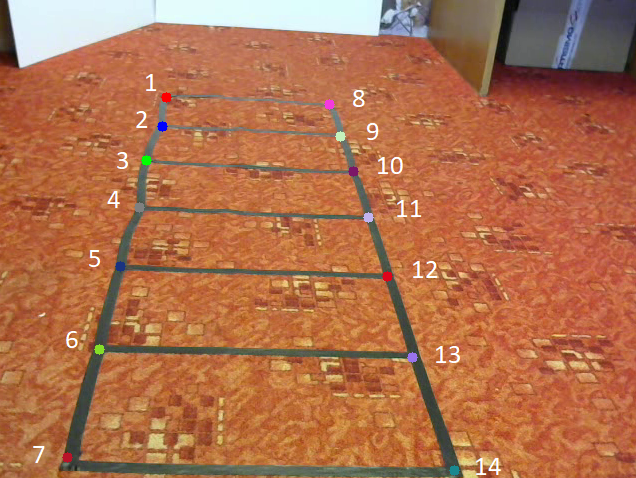
\includegraphics[width=0.8\linewidth]{img/experiments/right-ladder-numbered.png}
\caption{Numbering the points}
\label{fig:ladder_numbered}
\end{figure}

\begin{figure}
\centering
\begin{subfigure}{0.48\linewidth}
	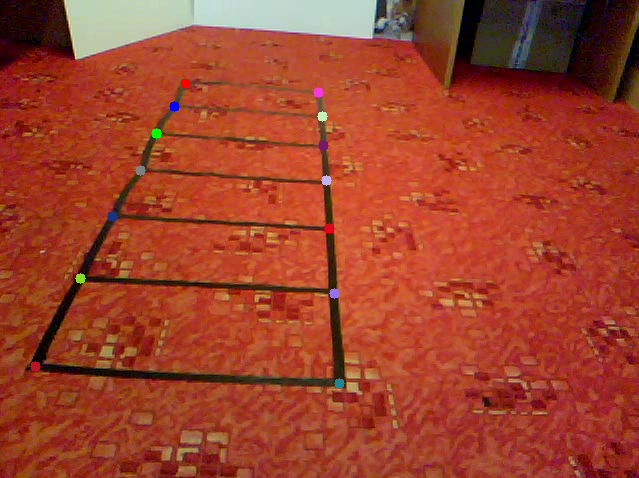
\includegraphics[width=\linewidth]{img/experiments/left-ladder.png}
\end{subfigure}
\begin{subfigure}{0.48\linewidth}
	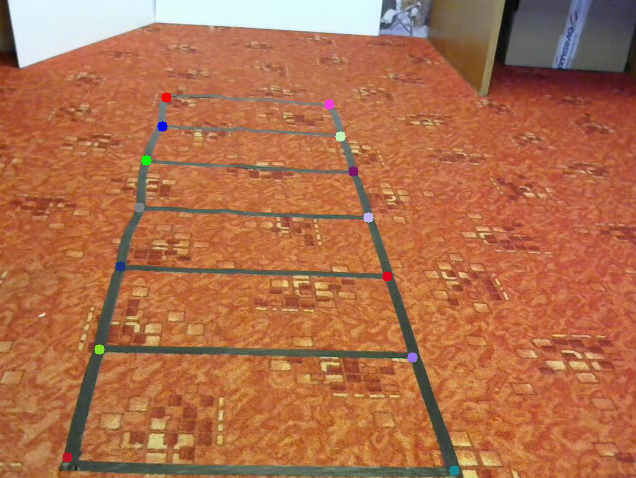
\includegraphics[width=\linewidth]{img/experiments/right-ladder.png}
\end{subfigure}
\caption{Selecting the points from the videos}
\label{fig:ladder_ground}
\end{figure}



\begin{figure}
\centering
\begin{subfigure}{0.48\linewidth}
	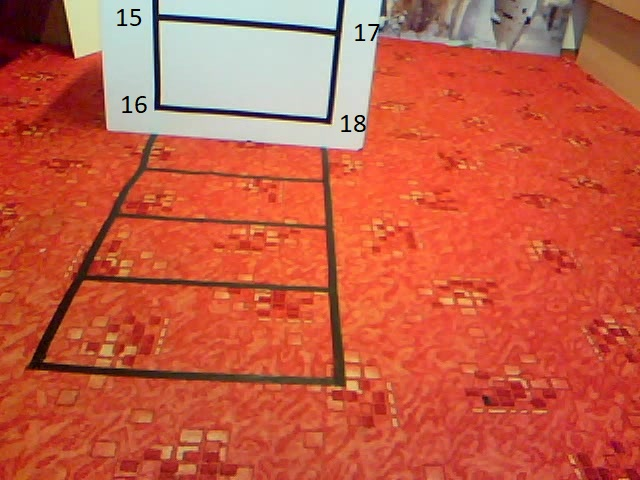
\includegraphics[width=\linewidth]{img/experiments/table-left.jpg}
	\caption{Left view of the camera with marks}
	\label{fig:tablenumbered}
\end{subfigure}
\begin{subfigure}{0.48\linewidth}
	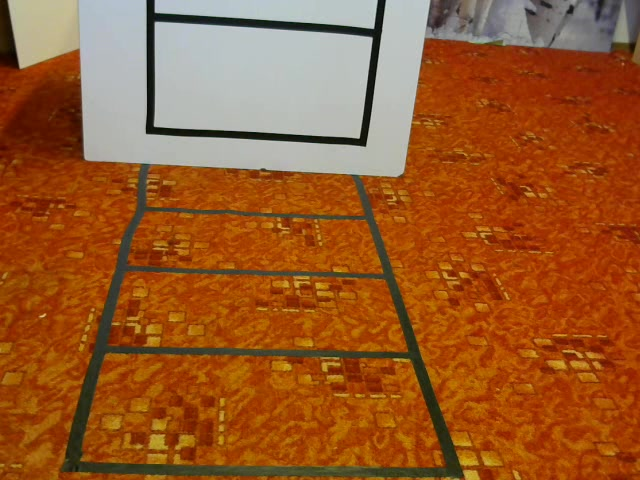
\includegraphics[width=\linewidth]{img/experiments/table-right.jpg}
	\caption{Right view of the camera}
\end{subfigure}
\caption{The views of the camera on the perpendicular plane to the ground}
\label{fig:table}
\end{figure}

\begin{figure}
\centering
\begin{tikzpicture}[]
	\draw (0, 0) -- (12, 0);
	\draw (0, 4) -- (12, 4);	
	\draw (0, 0) -- (0, 4);
	\draw (2, 0) -- (2, 4);
	\draw (4, 0) -- (4, 4);
	\draw (6, 0) -- (6, 4);
	\draw (8, 0) -- (8, 4);
	\draw (10, 0) -- (10, 4);
	\draw (12, 0) -- (12, 4);
	\node [right] at (0.1, -0.25) {200mm};
	\node [right] at (2.1, -0.25) {200mm};
	\node [right] at (4.1, -0.25) {200mm};
	\node [right] at (6.1, -0.25) {200mm};
	\node [right] at (8.1, -0.25) {200mm};
	\node [right] at (10.1, -0.25) {200mm};
	\node [right] at (12.1, 2) {400mm};
\end{tikzpicture}
\caption{Pattern used for experiments}
\label{fig:grid}
\end{figure}

\section{Complex experiments}

As the last step, we decided to test whole system in a real environment. This
time we included all parts of the application -- calibration, tracking and also
localization. In the previous experiments, we tested the liability of the
trackers and the precision of the results. Now we test the usability of the
system as the whole.

\subsection{Experiment with the one small object}

The most important experiment -- the experiment which decides if the system is
usable -- is experiment under real conditions. We created for our autonomous
robot a square to follow, with the length of the side equal 14.5~cm (see figure
\ref{fig:robot-square}). The robot did four laps around the square. The
results are displayed in the figure \ref{fig:square-results}.

We can see in the left picture, that the drawn line is similar to our shape.
Not having sharp edges, since our robot make a small arc. On the other hand,
the results from the another view are not so amazing. The coordinates have a
lot of noise over Z-axis. The noise is only present, if the robot is following
horizontal lines of the square. As the last step we computed maximum of the
distances between any two points, which were located. In this case, the ideal
value would be the length of the diagonal, which is equal to 20.5061~cm. Our
results are between 18.54~cm to 19.38~cm, depending on the run. That means,
that the error is only usually between 1 and 2~cm.

\begin{figure}
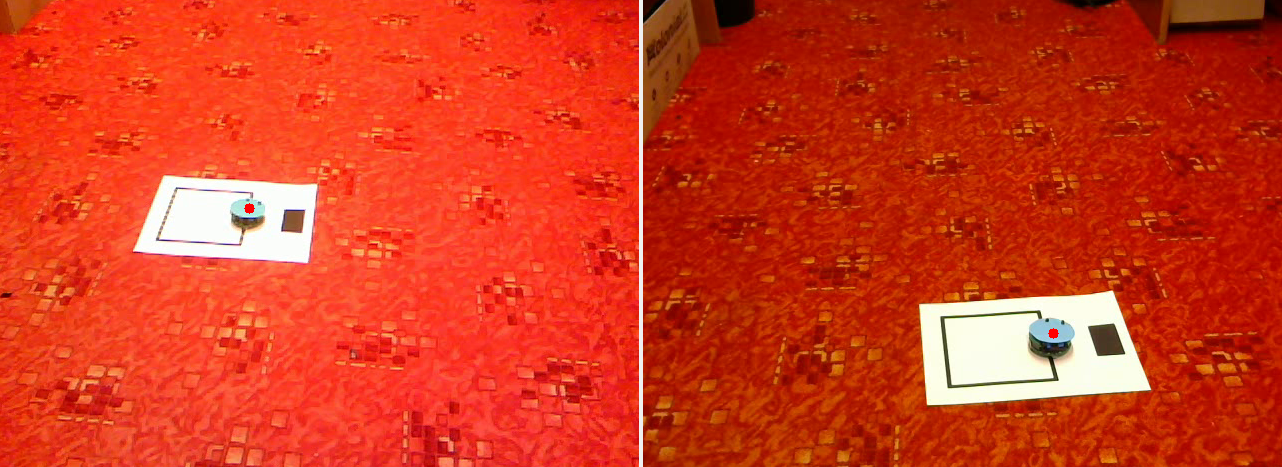
\includegraphics[width=\linewidth]{img/experiments/square-robot.png}
\caption{Experiment with the robot}
\label{fig:robot-square}
\end{figure}

\begin{figure}
\centering
\begin{subfigure}{0.48\linewidth}
	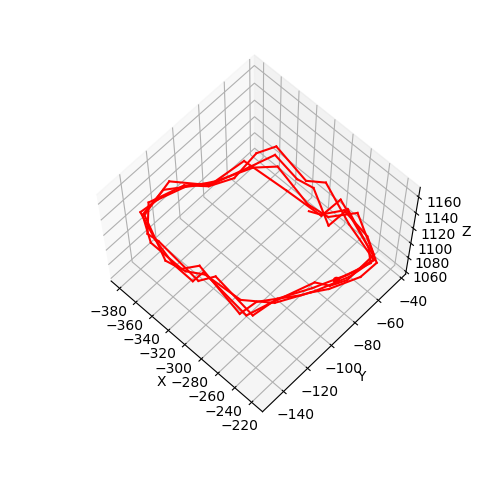
\includegraphics[width=\linewidth]{img/experiments/square-nice.png}
\end{subfigure}
\begin{subfigure}{0.48\linewidth}
	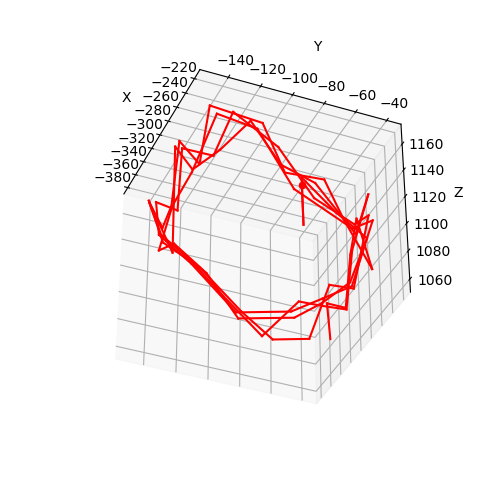
\includegraphics[width=\linewidth]{img/experiments/square-ugly.png}
\end{subfigure}
\caption{Results of the localization -- four laps by the robot}
\label{fig:square-results}
\end{figure}

\subsection{Experiment with two objects}

This experiment will test the ability of the system to track multiple objects.
This effectively exclude \simback{} tracker as it is not able to track multiple
objects. Furthermore, we track objects with multicolored surface, making \hsv
tracker also unusable. The rest of the trackers are mostly slower, more
problematic.

We can see the setup for the experiment in the figure \ref{fig:two-init}. We
can see two boxes, both in shades of blue. During testing many trackers failed
to track the object and lost it. We chose the \corr{} tracker as it provided
best results. It is medium fast tracker. The tracker sometimes lost the
images, but most of the time it was able to track. Because of the object lost,
sometimes an interaction of the user is needed, to reinitialize a tracker.

Sample results of the trajectories for two objects is displayed in the figure
\ref{fig:two-trajectories}. During the experiment, the boxes were moving
between the yellow marks and swapped places. We can see these four marks also in
both trajectories quite close to each other. 

\begin{figure}[p]
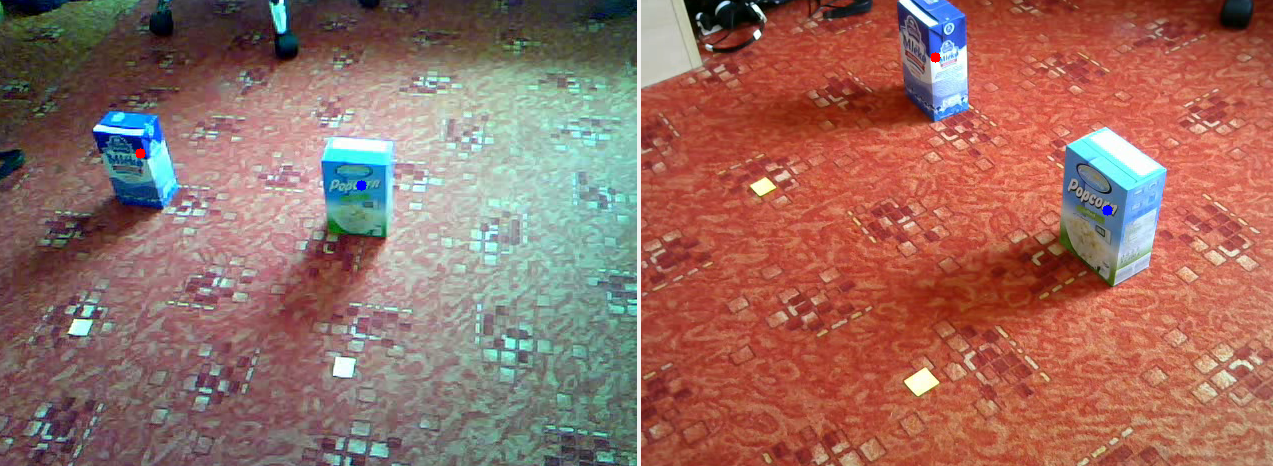
\includegraphics[width=\linewidth]{img/experiments/two-objects.png}
\caption{Initialization of the two objects}
\label{fig:two-init}
\end{figure}

\begin{figure}
\centering
\begin{subfigure}{0.48\linewidth}
	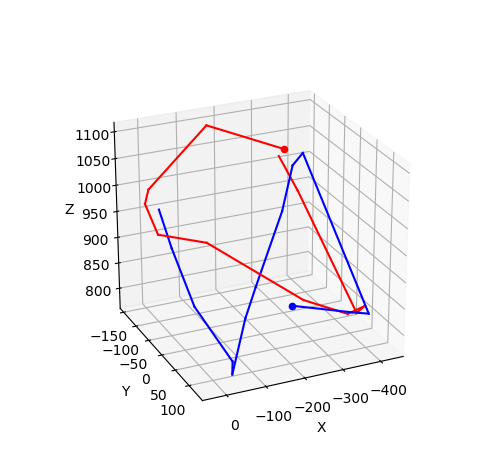
\includegraphics[width=\linewidth]{img/experiments/trajectories1.png}
\end{subfigure}
\begin{subfigure}{0.48\linewidth}
	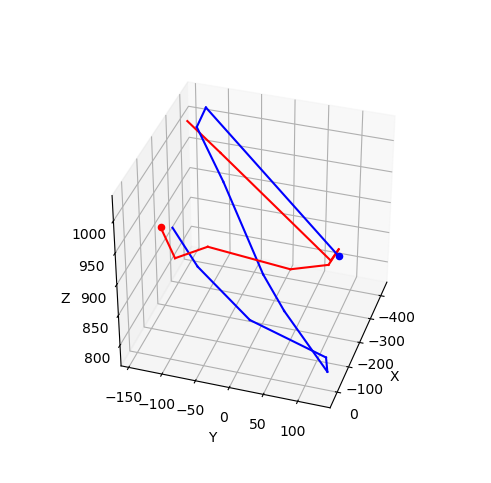
\includegraphics[width=\linewidth]{img/experiments/trajectories2.png}
\end{subfigure}
\caption{Sample trajectories from tracking two objects}
\label{fig:two-trajectories}
\end{figure}
